%%%%% Dokumentacia IFJ Projekt %%%% 
%% Autor: Albert Groma

\documentclass[a4paper,11pt]{article}
\usepackage[slovak]{babel}
\usepackage[left=1.5cm,text={18cm, 25cm},top=2.5cm]{geometry}
\usepackage{times}
\usepackage[czech,ruled,noline,longend,linesnumbered]{algorithm2e}
\usepackage{csquotes}
\usepackage[utf8]{inputenc}
\usepackage{titling}
\usepackage[hidelinks]{hyperref}
\usepackage{latexsym}
\usepackage{multirow}
\usepackage{diagbox} 
\usepackage{subcaption}
\usepackage{graphicx}
\graphicspath{{images/}}

\bibliographystyle{czplain}

\begin{document}	
	\begin{titlepage}
		\begin{center}
			
\includegraphics[width = 10cm]{logo_cz.png}\\
			\vspace{\stretch{0.382}}
			\LARGE{\bfseries Implementácia prekladaču imperatívneho jazyka IFJ20}\\[2mm]
			\LARGE{Dokumentácia k projektu}\\[5mm]
			\Large{ Tím 141, varianta I}\\
			\vspace{\stretch{0.418}}
			\begin{table}[h]
				\begin{center}
					\Large
					\begin{tabular}{lll}
						\multicolumn{2}{l}{\bfseries Vedúci tímu:} & \\[1mm]
						\hspace{5mm} & Fabo Adam  (xfaboa00) & 25\% \\[1mm]
						\multicolumn{2}{l}{\bfseries Ostatní členovia tímu:} & \\[1mm]
						\hspace{5mm} & Groma Albert  (xgroma00) & 25\% \\[1mm]
						\hspace{5mm} & Gabriš Stanislav (xgabri18) & 25\% \\[1mm]
						\hspace{5mm} & Országh Roman  (xorsza01) & 25\% \\[1mm]
					\end{tabular}
				\end{center}
			\end{table}
			\vspace{\stretch{0.200}}
		\end{center}
		\begin{minipage}{.45\linewidth}
			\begin{flushleft}
  				{\Large 4. December 2020}
			\end{flushleft}
		\end{minipage}
		\begin{minipage}{.45\linewidth}
    		\begin{flushright}
      			{\Large Rozšírenia: \hspace{5mm} - \hspace{5mm}}
    		\end{flushright} 
  		\end{minipage}
	\end{titlepage}

	\tableofcontents
	\thispagestyle{empty}
	\cleardoublepage

	\setcounter{page}{1}

	\section{Úvod}\label{sec:uvod}

		\noindent V prekladači využívame priame generovanie kódu, t.j. generácia kódu prebehne vždy, keď má program dostatok informácii na to, aby vygeneroval inštrukcie. Lenže nie vždy program po spracovaní tokenu vie, aký kód má generovať, preto v kóde využívame zásobníky.\\

		\noindent Štruktúra nášho kompilátora je nasledovná:
		\begin{figure}[h]
			\centering
			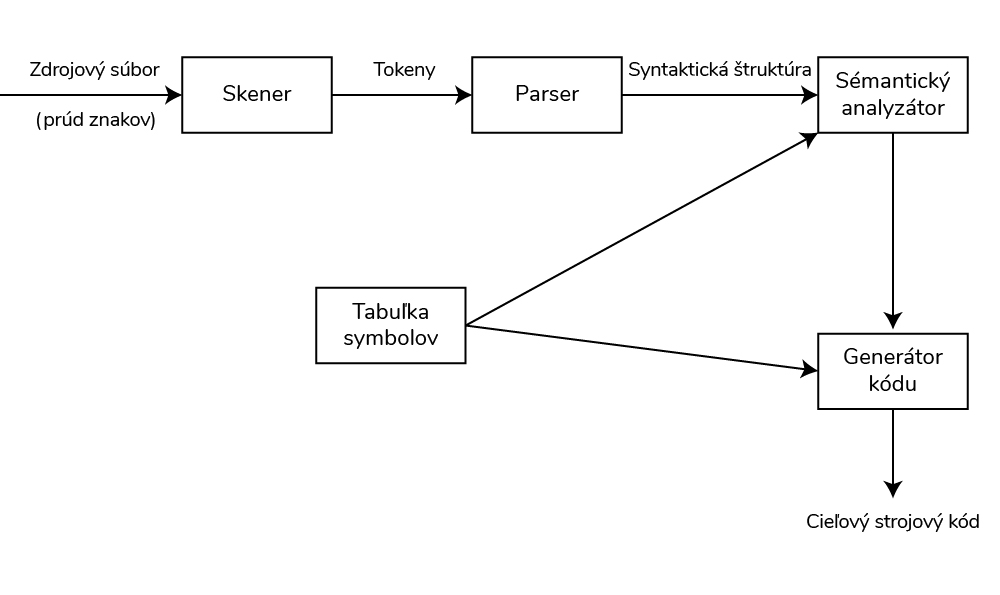
\includegraphics[width = 12cm]{Compiler.jpg}\\
			\caption{Schéma prekladača}
			\label{fig:compilator}
		\end{figure}

	\section{Lexikálna analýza}\label{sec:lexi}

		Lexikálny analyzátor dostane od parseru prázdny token, ktorý sa snaží naplniť a vrátiť. Skúma vstup podľa navrhnutého konečného automatu. Ak narazí na znak ktorý už podľa KA nemôže spracovať, vráti ho pomocou funkcie ungetc() naspäť. Aj v niektorých iných prípadoch pužívame funkciu ungetc(), ako napríklad pri prechode zo stavu 1 do stavu štart v konečnom automate (viz obr. \ref{fig:diaglex1} a obr. \ref{fig:diaglex2} v prílohe).\\
		Následne podľa pravidiel v KA buď vracia naplnený token alebo vracia LEXICAL\_ERROR, ak sa nenachádza v konečnom stave. Token drží v type základnú informáciu o lexéme a v data dodatočné informácie. Lexikálny analyzátor nemá prístup k tabuľke symbolov. Keďže lexikálny analyzátor nepozná momentálny kontext nevedel by (v našom riešení) správne pracovať s danou tabuľkou.\\
		Pri blokovom komentáry sme sa rozhodli, ak sa vyskytuje, posielať aj informáciu o NEWLINE (podľa nasledujúcich znakov), inak po prečítaní komentáru pokračujeme v lexikálnej analýze od znova (podľa KA).

	\section{Parser}\label{sec:parser}

		Parser vytvorí token a pošle ho lexikálnemu analyzátoru, ktorý ho naplní pričom, ak vznikne error, tak parser ukončuje program. Všetky tokeny, ktoré sa načítajú sa ukladajú do globálneho zásobníka (toto rozhodnutie padlo na začiatku vývoja kompilátora, keď sme ešte nevedeli, či náhodou nebudeme potrebovat predchádzajúce tokeny). Parser obsahuje okrem funkcii, ktoré predstavujú neterminály v pravidlách, taktiež 2 špeciálne funkcie a to match() a get\_next\_token(). \\ \\
		Predstavme si, že nastane situácia kedy očakávame neterminál “)”. Na toto je vytvorená funckia match(RPAREN) (RPAREN je súčasťou enumu), ktorá načíta ďalší token a overí, či ďalší token je naozaj pravá zátvorka, pričom ho “potvrdí (ak je, tak vracia NO\_ERROR, ak nie je, tak vracia SYNTAX\_ERORR). Nastávajú aj situácie, kedy musíme načítať token a podľa typu tokena sa rozhodnúť, ktoré pravidlo vybrat. Tam používame funkciu get\_next\_token(), ktorá načíta ďalší token, ale “nepotvrdí" ho.  Funkcia get\_next\_token() načíta najviac jeden token, aj keď je volaná viackrát a ak je po tejto funkcii volaná funkcia match(), tak nenačítava sa ďalší token, ale “potvrdí” už prednačítaný token. \\
	
	\section{Tabuľka symbolov}\label{sec:tabulka}

		Podľa zadania sme implementovali tabuľku symbolov ako tabuľku binárneho vyhľadávacieho stromu. Táto tabuľka slúži na uchovávanie identifikátorov a~funkcií, ktoré sa v~programe definujú. Každý symbol sa definuje buď ako identifikátor alebo funkcia. Podľa toho o~aký typ symbolu ide sa využívajú jednotlivé funkcie na prácu s~tabuľkou. Všetky potrebné informácie o~daných symboloch sú uložené v~univerzálnej štruktúre uzla, ktorý sa používa ako pre identifikátory, tak aj pre funkcie.\\

		\begin{figure}[h]
			\centering
			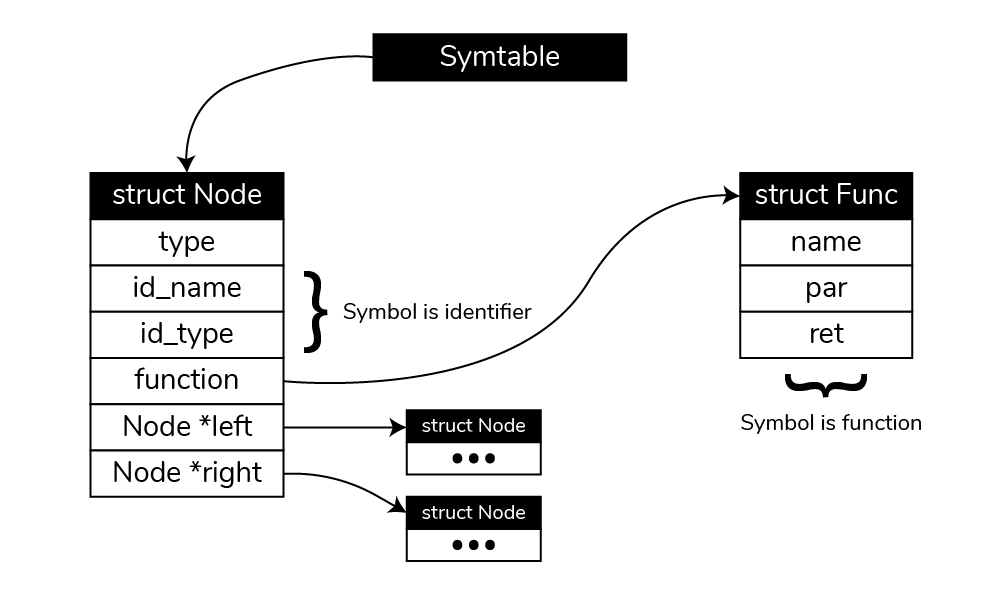
\includegraphics[width = 12cm]{Symtable.jpg}\\
			\caption{Tabuľka symbolov}
			\label{fig:symtable}
		\end{figure}

		\noindent Pre jednoduchšiu a~efektívnejšiu prácu sme vytvorili globálnu tabuľku pre všetky funkcie a~pre identifikátory samostatné tabuľky. Tieto samostatné tabuľky sa vytvoria zakaždým, keď nastane vnorenie do funkcie, cyklu, podmienky apod. Tabuľky sa vždy ukladajú do zásobníku tabuliek. Týmto zabezpečíme, aby sme mali „scope“ jednotlivých identifikátorov pod kontrolou. Po vynorení zo „scope“ sa tabuľka automaticky vymaže a~de-alokuje sa všetka alokovaná pamäť.\\

		\noindent Implementovali sme niekoľko funkcií, potrebných na prácu so stromom: inicializácia binárneho stromu, zrušenie binárneho stromu, pridanie identifikátora, pridanie funkcie, vyhľadanie identifikátora/funkcie na základe názvu. Odstránenie jednotlivých položiek nebolo potrebné vzhľadom na implementáciu projektu, keďže nie je potrebné funkcie a~ani identifikátory vymazávať. Na konci prekladu sa spustí ešte samostatná de-alokácia tabuliek, ktoré neboli vymazané, aby sme zamedzili memory leak-u.\\

	\section{Sémantická analýza a generovanie kódu}\label{sec:sem} 
		Sémantické akcie sú vkladané medzi akcie parsera pričom neovplyvňujú parser, iba spracuvávaju načítané tokeny.\\
		Ako už bolo napísané v úvode, v programe negenerujeme ASS ale používame priame generovanie kódu.\\
		Pri generovaní kódu naplno využívame dátový zásobník inštrukčnej sady, ktorý výrazne uľahčil prácu pri generovaní kódu, hlavne pri výrazoch (\ref{subsec:vyrazy}).\\
		V nasledujúcich častiach sú vysvetlené jednotlivé príkazy a spôsoby, ktorými ich spracúvavame.\\
	
		\subsection{Príkaz priradenia}\label{subsec:prirad}

		Na to aby sme mohli spracovať tento príkaz, musíme ho celý načítať, čo znamená že hodnoty  musíme niekde priebežne ukladať a na to nám slúžia zásobniky.\\
		Identifikátory postupne načítavame do zásobniku pričom overujeme či existujú už v tabuľke symbolov. Keď sa dostaneme na koniec príkazu, tak ešte musíme ošetriť typy a ich počet, pričom na to slúži druhý zásobnik, ktorý sa naplní pri tom ako sa vyhodnocujú výrazy.\\ Vyhodnotenie výrazov zaručuje, že výsledok výrazu bude uložený na dátovom zásobniku, a tým padom je už iba potrebné vybrať hodnoty zo zásobníku v opačnom poradí.\\
		Viz obr. \ref{fig:3}.2 v prílohe.
	
		\subsection{Definícia premennej}\label{subsec:defprem}

		Funguje takmer rovnako ako príkaz priradenia (\ref{subsec:prirad}) až na to, že treba zavolať inštrukciu DEFVAR a uložiť identifikátor do tabuľky symbolov. Viz obr. \ref{fig:4}.4 v prílohe.
	
		\subsection{Definicia funkcie}\label{subsec:deffun}

		Pri spracovaní funkcie sa načíta a uloží meno do premennnej, parametry do zásobníka parametrov a return values do zásobníka return values. Ak sú tieto hodnoty vporiadku (meno funkcie ešte neexituje v tabuľke symbolov, parametry nemajú rovnaké identifikátory), tak sa uloží táto funkcia do tabuľky symbolov a vytvára sa nový strom v zásobníku stromov (viac pri tabulke symbolov (\ref{sec:tabulka})). Parametre predávame funkcii cez dátový zásobník v inštručnej sade.\\
		Viz obr. \ref{fig:4}.2 a volanie funkcie Viz obr. \ref{fig:4}.3 v prílohe.

		\subsection{Podmienený príkaz (if-else)}\label{subsec:ifelse}
		
		If očakáva, že výraz bude boolovského typu, overiť sa to dá zo zásobníku, kam sa uloží typ výrazu a podľa toho sa skáče na návestia.\\
		
		\noindent Problém, ktorý tu vzniká pri viacerých použitiach if-och alebo pri zanorených if-och, je aby sa návestia neopakovali.\\ Toto sme zase vyriešili pomocou zásobníku, do ktorého sa pushne číslo if-u (toto číslo sa každým if-om inkrementuje), a keď dôjde na koniec if-u, tak sa toto číslo pop-ne a vytvorí korektné náveštie.\\
		Viz obr. \ref{fig:3}.1 v prílohe.

		\subsection{For cyklus}\label{subsec:for}
		
		For cyklus je svojou konštrukciou podobný if-u, len komplikovanejší.\\

		\noindent Na kóde v prílohe na obr. \ref{fig:4}.1 v prílohe. si môžete povšimnúť rôzne rozsahy platnosti a taktiež spôsob riešenia toho, že v hlavičke if-u prebieha deklarácia iba raz. Taktiež ako pri if-e, existuje zásobník integerov, pomocou ktorých sa generujú náveštia.

		\subsection{Rámce}\label{subsec:ramce}

		\noindent Rôzne rozsahy platnoti riešime tak ako je to napísané pri TS, a to tak, že máme zásobník stromov, pričom unikátne meno premennej je zložené z jej identifikátora a čísla, ktoré určuje poradie stromu v zásobníku. Pri začiatku nového rozsahu platnosti sa všetky premenné, ktoré boli doteraz vytvorené push-nu na dátový zásobník, vytvorí sa nový frame, definuju sa všetky premenné a potom sa pomocou pop-ov nahrajú hodnoty do premenných.\\ Na konci rozsahu sa pop-ne posledný strom a všetky deklarované premenné sa push-nu, vymaže sa frame a popopujú sa hodnoty naspäť. Názorne je to vysvetlené na príklade v prílohe, viz obr. \ref{fig:3}.3. Je nám jasné že takáto konštrukcia nie je legálna v ifj20, ale znázorňuje riešenie napr. pri vnorených if-och bez toho aby ukážkový kód bol zbytočne dlhý.

		\subsection{Sémantické akcie pri returne}\label{subsec:return}

			\noindent Pri objavení sa returnu vo funkcií sa po vyhodnotení expressions (return expression,expression,...) naplní zásobník typov a kontroluje sa, podla hlavičky funkcie, či sedí počet návratových hodnôt a správnosť ich typov. Tieto hodnoty sa v generovanom kóde pushujú po čom sa podľa zanorenia popujú framy.
			\noindent Zanorenie sa zisťuje zo zásobníku stromov.\\

			\noindent Kontrola výskytu returnu:

			\noindent Po konci funkcie sa kontroluje či funkcia mala return (pomocou globálnej premennej ret\_flag, ktorá je buď 1(return present) alebo 0 (return not present)) a či by funkcia mala mať return (return typy v hlavičke)).\\

		\subsection{Výrazy}\label{subsec:vyrazy}

			Výrazy spracúvame pomocou precedenčnej tabuľky (\ref{subsec:prectab}). Pri spracovaní používame zásobník, na ktorý si ukladáme znaky, ktoré reprezentujú jednotlivé tokeny a postupujeme podľa algoritmu zdola navrh, ktorý bol preberaný na prednáškach.\\

			\noindent Na začiatku, pred spracovaním výrazov si overujeme spätne, či posledný overený token (matched token) je identifikátor, ak áno, tak ho pridáme do spracovania výrazov, ak nie, tak sa pokračuje. Takýmto spôsobom riešime volanie funkcie. Čiže \enquote{ID} ide na volanie funkcie, ale ak je \enquote{ID} a za identifikátorom nie je zátvorka, tak ide do vyhodnotenia výrazov, kde pridá ten identifikátor).\\

			\noindent So zásobníkom pracujeme ako so stringom, kde podľa priority operátorou (precedenčnej tabuľky) určujeme, ktorá z možností \textless, \textgreater, = alebo chyba sa má vykonať.\\

			\noindent Pri možnosti \textless\quad vkladáme znak \enquote{\textless}\quad na zásobník a potom pri \textgreater\quad zisťujeme akému pravidlu sa rovná to, čo je za znakom \enquote{\textless}, buď skončíme s chybou alebo daným pravidlom, pomocou ktorého generujeme priamo kód. \\

			\noindent Typ výrazu ukladáme na zásobník, kde si ho potom overujú iné časti programu.

		\subsection{Optimalizácie}\label{subsec:opt}
			V kode sme nerobili žiadne optimalizácie, tým pádom samostatný generovaný kód bude pomalý, ale za to, je generácia kódu ľahšia.

	\section{Práca v tíme}\label{sec:tym}

		\subsection{Rozdelenie práce}\label{subsec:rozpra}
		\begin{table}[h]
		\begin{center}
			\begin{tabular}{|l|l|}
				\hline
				\bfseries Člen tímu &
				\bfseries Rozdelenie práce \\ \hline
				\multirow{2}{*}{Fabo Adam  (xfaboa00)} & organizácia práce, zavedenie štruktúry projektu, syntaktická analýza,\\
				&sémantická analýza, generovanie kódu, testovanie , dokumentácia\\
				\multirow{2}{*}{Groma Albert  (xgroma00)} & syntaktická analýza, syntaktická analýza výrazov, generovanie kódu,\\
				&sémantická analýza, testovanie, dokumentácia\\
				\multirow{2}{*}{Gabriš Stanislav (xgabri18)} & lexikálna analýza, generovanie kódu, testovanie, sémantická analýza,\\
				&dokumentácia\\ 
				\multirow{2}{*}{Országh Roman  (xorsza01)} & príprava štruktúr a zásobníkov, generovanie kódu, sémantická analýza,\\
				&testovanie, dokumentácia\\ \hline
			\end{tabular}
			\caption{Tabulka rozdelenia práce}
			\label{tab:rozprac}
		\end{center}
		\end{table}
	\section{Záver}\label{sec:zaver}

	\noindent Pri riešeni projektu sme si rozšírili skúsenosti s prácou v týme a taktiež sme nabrali množstvo praktických vedomostí. Vypracovavali sme projekt pomocou informácii, ktoré nám poskytli predmety IFJ a IAL, ale taktiež sme sa inšipirovali knihami Crafting a Compiler with C\cite{Fischer:1991} a Algoritmy a štruktúry údajov\cite{Wirth:1988}.\\

	\cleardoublepage
	\section{Prílohy}\label{sec:prilohy}

		\subsection{Generovanie kódov}\label{subsec:genkod}
			\begin{figure}[h!]
				\centering
				\begin{subfigure}[h]{0.4\textwidth}
	    			\centering
	    			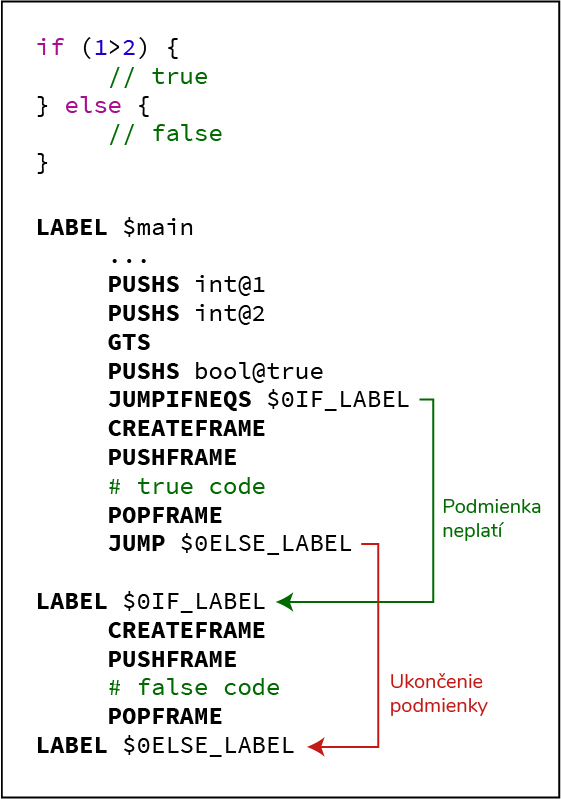
\includegraphics[width=\textwidth]{codes/if.jpg}\\
					\caption*{Obr. 3.1: Podmienený príkaz (if-else)}
					\label{fig:if}
					\vspace{2cm}
					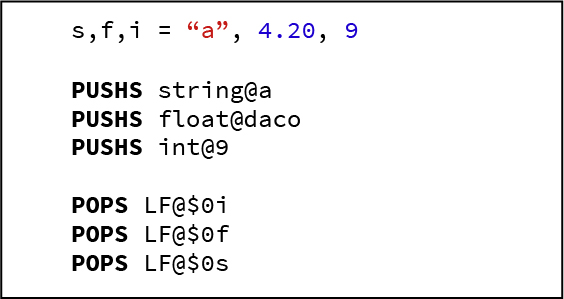
\includegraphics[width=\textwidth]{codes/multi_var.jpg}\\
					\caption*{Obr. 3.2: Príkaz priradenia}
					\label{fig:prir}
				\end{subfigure}\qquad
				\begin{subfigure}[h]{0.4\textwidth}
					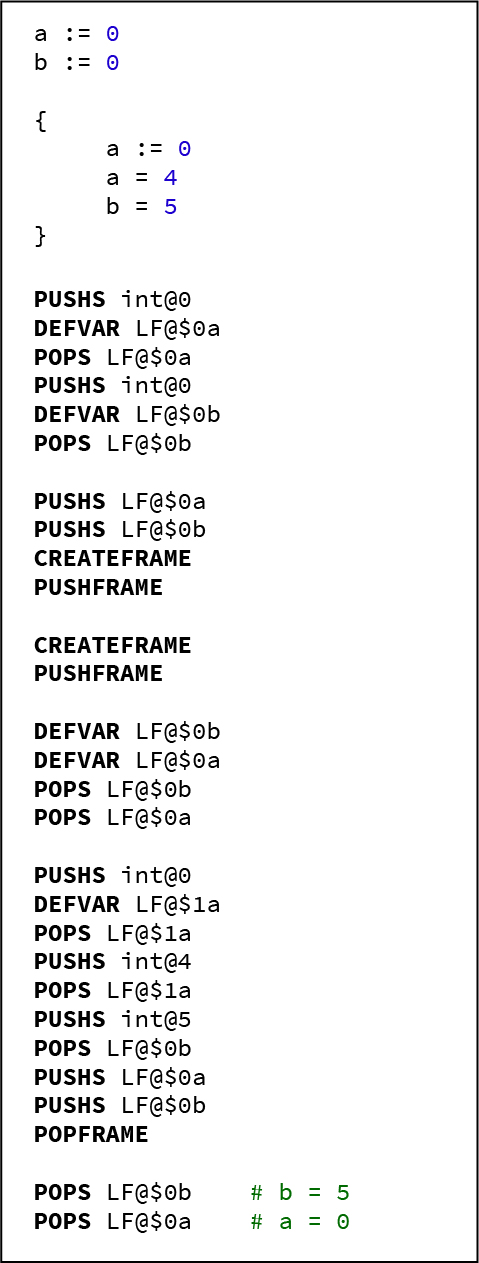
\includegraphics[width=\textwidth]{codes/ramce.jpg}\\
					\caption*{Obr. 3.3: Rámce}
					\label{fig:ramce}
				\end{subfigure}
				\caption{Generovanie kódov časť 1.}
				\label{fig:3}
			\end{figure}
			\cleardoublepage
			\begin{figure}[h!]
				\centering
				\begin{subfigure}[h]{0.4\textwidth}
					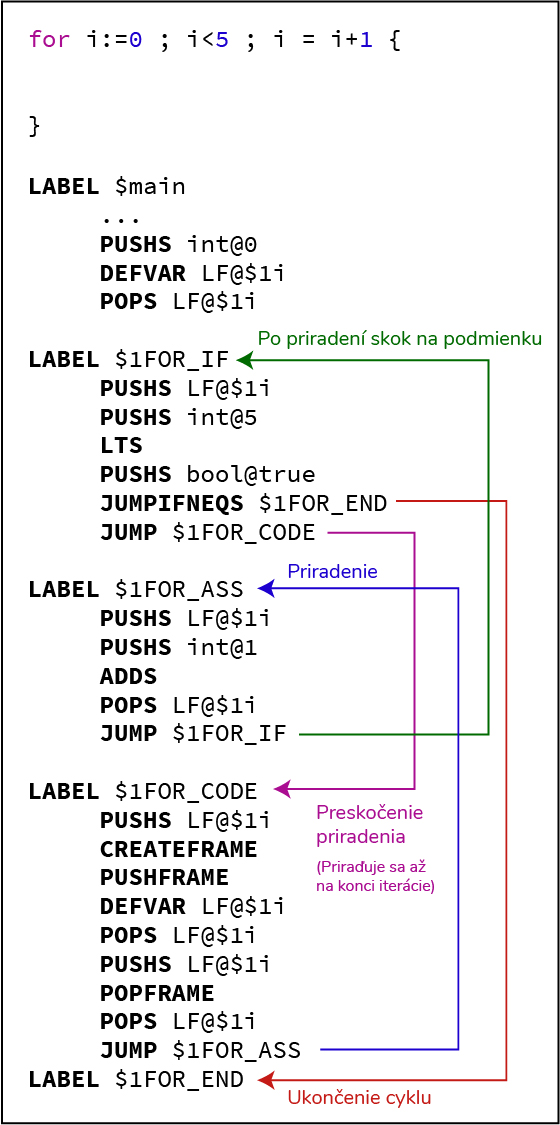
\includegraphics[width=\textwidth]{codes/for.jpg}\\
					\caption*{Obr. 4.1: For cyklus}
					\label{fig:for}
				\end{subfigure}\qquad
				\begin{subfigure}[h]{0.4\textwidth}
	    			\centering
	    			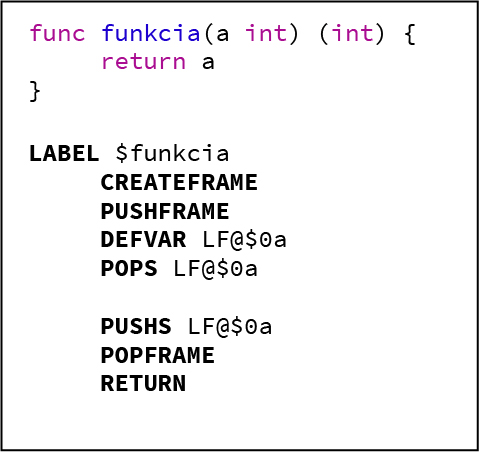
\includegraphics[width=\textwidth]{codes/func.jpg}\\
					\caption*{Obr. 4.2: Definícia funkcie}
					\label{fig:funcdef}
					\vspace{1cm}
	    			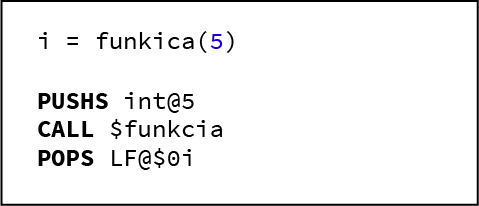
\includegraphics[width=\textwidth]{codes/func_call.jpg}\\
					\caption*{Obr. 4.3: Volanie funkcie}
					\label{fig:funccall}
					\vspace{1cm}
					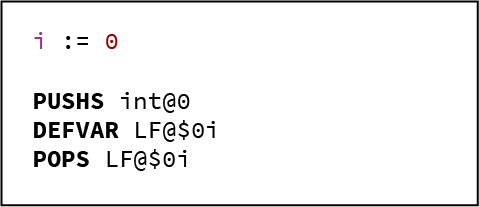
\includegraphics[width=\textwidth]{codes/declaration.jpg}\\
					\caption*{Obr. 4.4: Deklarácia}
					\label{fig:deklaracia}
				\end{subfigure}
				\caption{Generovanie kódov časť 2.}
				\label{fig:4}
			\end{figure}
			\cleardoublepage

		\subsection{Diagram konečného automatu zameraný na lexikálny analyzátor}\label{subsec:lexauto}

			\begin{figure}[h]
				\centering
				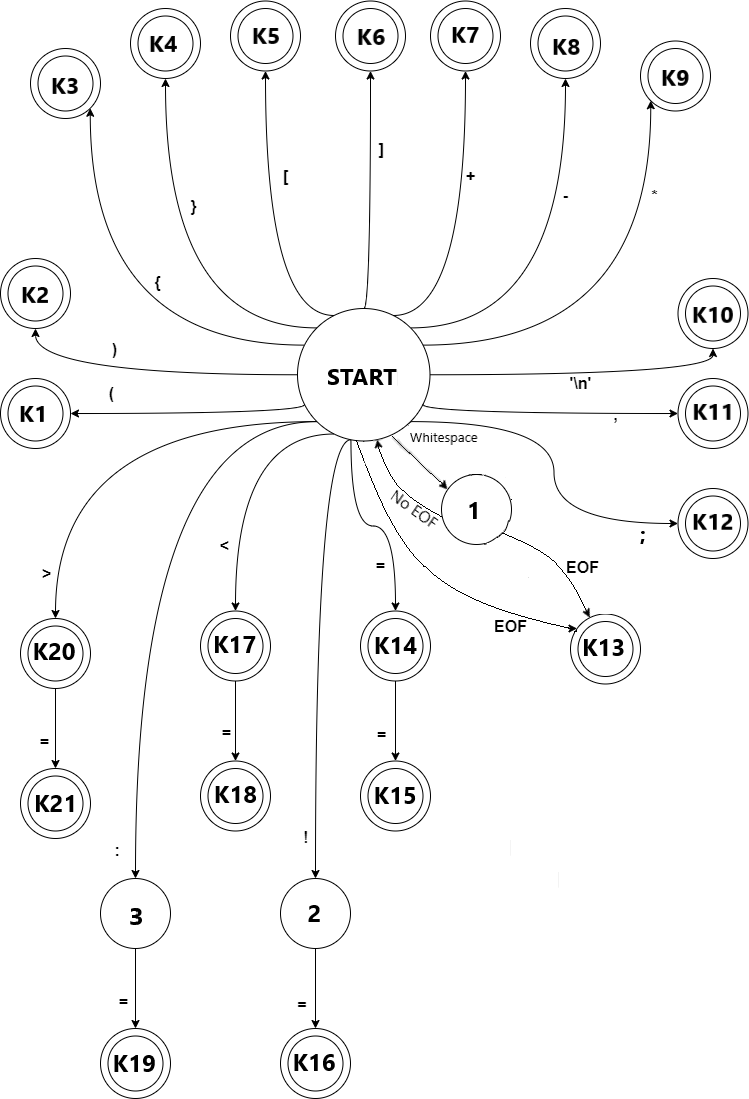
\includegraphics[width = 10cm]{LA_KA_1.png}\\
				\caption{Diagram konečného automatu zameraný na lexikálny analyzátor časť 1.}
				\label{fig:diaglex1}
			\end{figure}

			\begin{figure}[h]
				\centering
				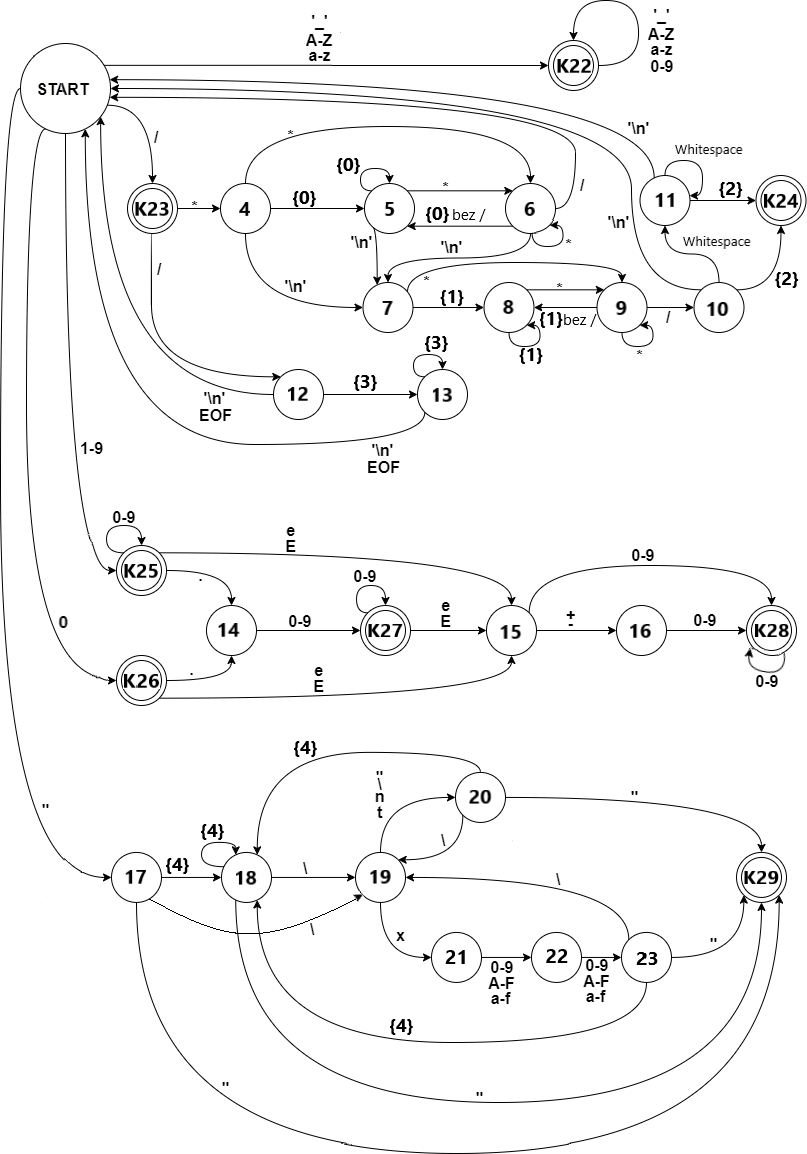
\includegraphics[width = 10cm]{LA_KA_2.png}\\
				\caption{Diagram konečného automatu zameraný na lexikálny analyzátor časť 2.}
				\label{fig:diaglex2}
			\end{figure}

			\begin{figure}[h]
				\centering
				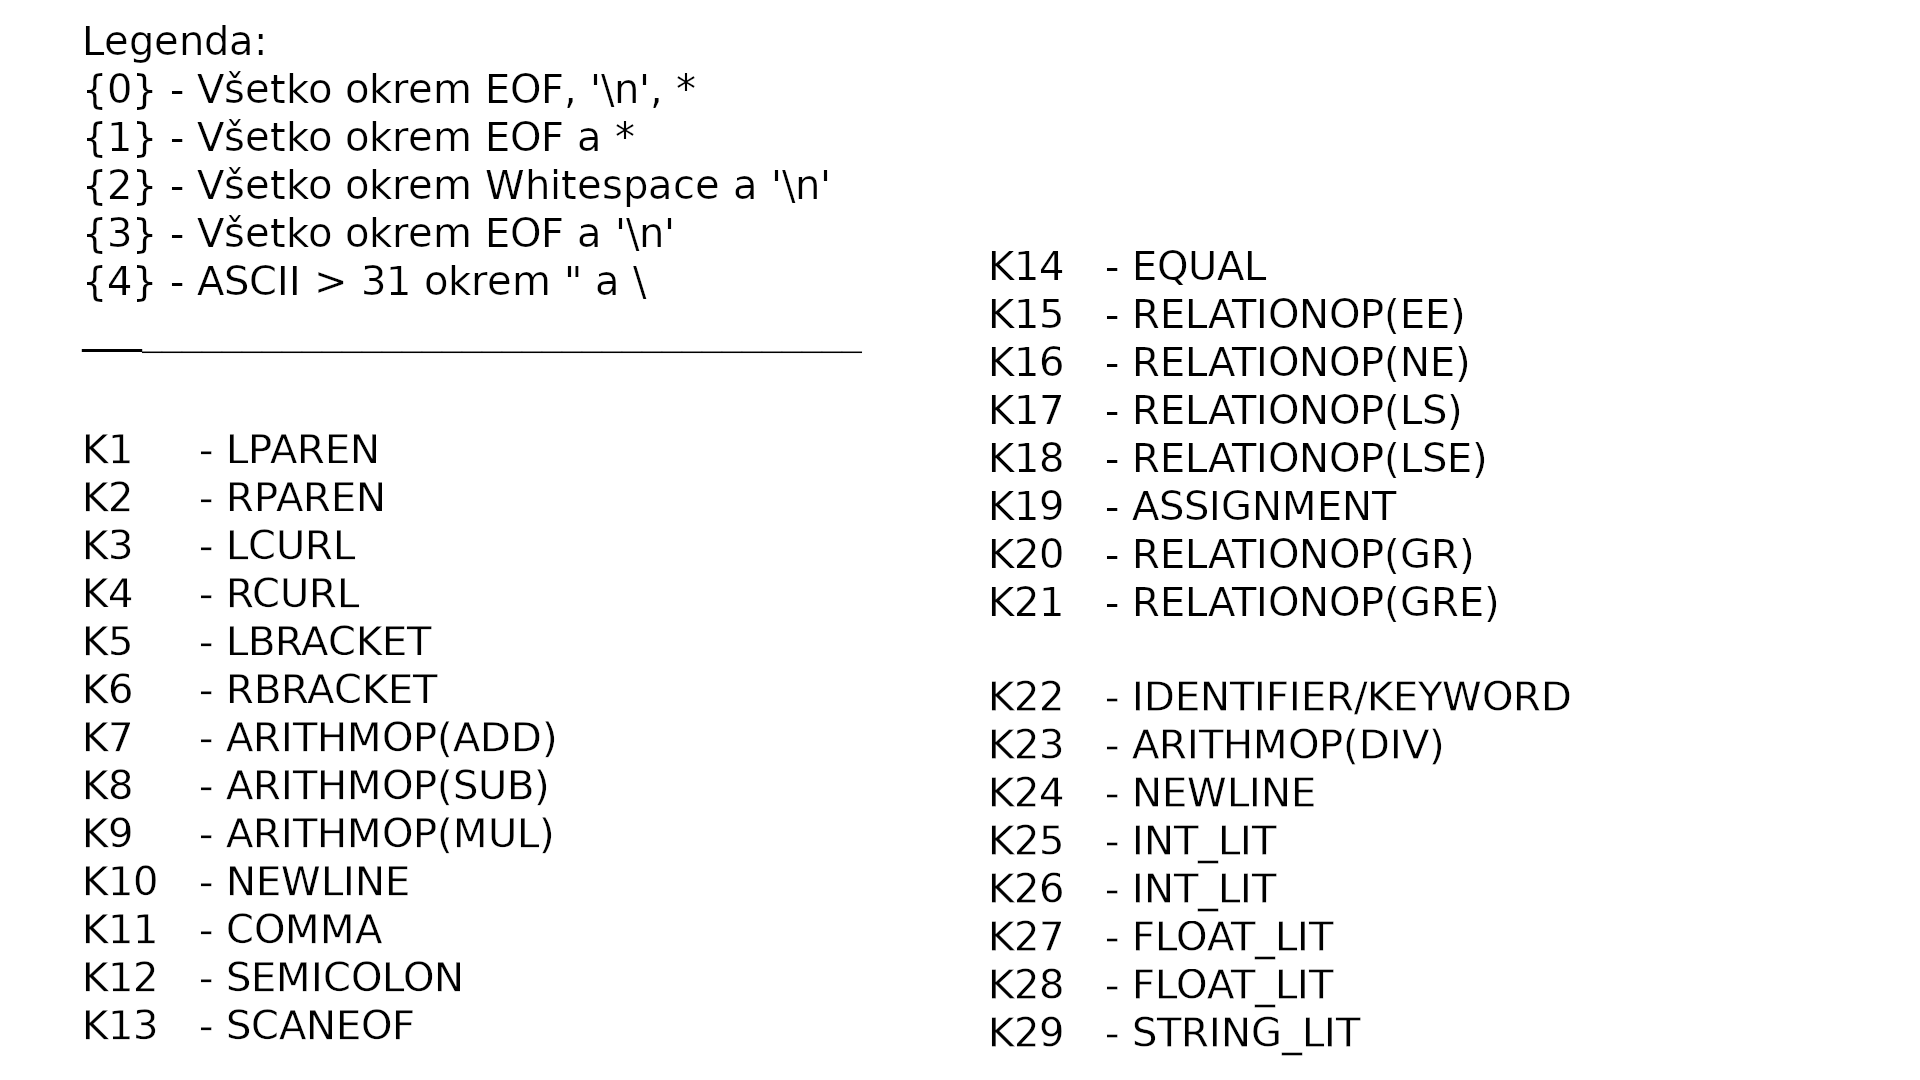
\includegraphics[width = 10cm]{legenda.png}\\
				\caption{Legenda ku diagramu konečného automatu}
				\label{fig:legenda}
			\end{figure}

		\cleardoublepage

		\subsection{LL Tabuľka}\label{subsec:lltable}

			\begin{figure}[h]
				\centering
				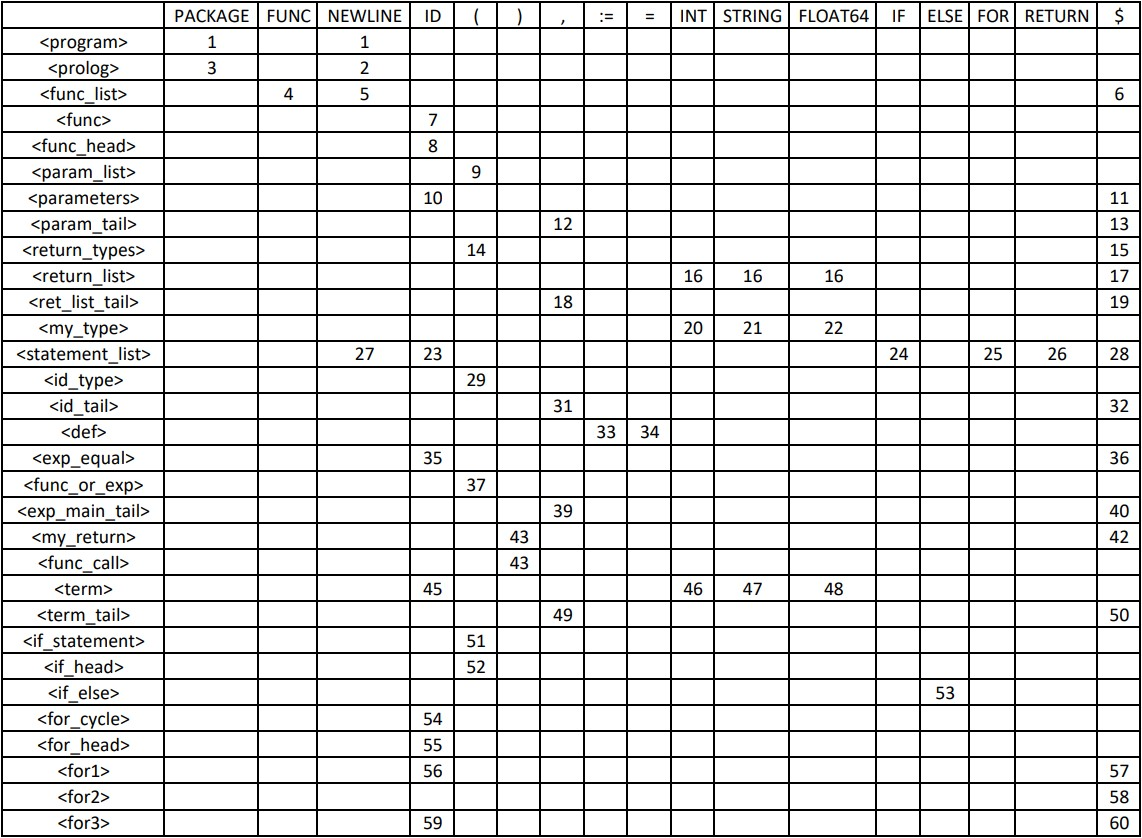
\includegraphics[width = 15cm]{LL_Tabulka.jpg}\\
				\caption{LL Tabuľka}
				\label{fig:lltable}
			\end{figure}
		\cleardoublepage
		\subsection{LL Gramatika}\label{subsec:llgram}
			\begin{table}[h!]
				\begin{center}
					\begin{scriptsize}
					\begin{tabular}{lll}
						1. &\textless program\textgreater & $\rightarrow$ \textless prolog\textgreater  \textless func\_list\textgreater  SCANEOF\\
					    2. &\textless prolog\textgreater 	   & $\rightarrow$ NEWLINE \textless prolog\textgreater \\
					    3. &\textless prolog\textgreater 	   & $\rightarrow$ package main NEWLINE\\
					    4. &\textless func\_list\textgreater 	   & $\rightarrow$ func \textless func\textgreater  \textless func\_list\textgreater \\
 						5. &\textless func\_list\textgreater 	   & $\rightarrow$ NEWLINE \textless func\_list\textgreater \\
    					6. &\textless func\_list\textgreater  	   & $\rightarrow$ $\varepsilon$\\
    					7. &\textless func\textgreater  		   & $\rightarrow$ \textless func\_head\textgreater  \textless statement\_list\textgreater  NEWLINE \} NEWLINE\\
    					8. &\textless func\_head\textgreater  	   & $\rightarrow$ ID \textless param\_list\textgreater  \textless return\_types\textgreater  \{ NEWLINE\\
    					9. &\textless param\_list\textgreater  	   & $\rightarrow$ ( \textless parameters\textgreater  )\\
    					10. &\textless parameters\textgreater  	   & $\rightarrow$ ID \textless type\textgreater  \textless param\_tail\textgreater \\
    					11. &\textless parameters\textgreater  	   & $\rightarrow$ $\varepsilon$\\
    					12. &\textless param\_tail\textgreater  	   & $\rightarrow$ , ID \textless type\textgreater  \textless param\_tail\textgreater \\
    					13. &\textless param\_tail\textgreater  	   & $\rightarrow$ $\varepsilon$\\
    					14. &\textless return\_types\textgreater 	   & $\rightarrow$ ( \textless return\_list\textgreater  )\\
    					15. &\textless return\_types\textgreater 	   & $\rightarrow$ $\varepsilon$\\
    					16. &\textless return\_list\textgreater 	   & $\rightarrow$ \textless my\_type\textgreater  \textless ret\_list\_tail\textgreater \\
    					17. &\textless return\_list\textgreater  	   & $\rightarrow$ $\varepsilon$\\
    					18. &\textless return\_list\_tail\textgreater & $\rightarrow$ , \textless my\_type\textgreater  \textless ret\_list\_tail\textgreater \\
    					19. &\textless return\_list\_tail\textgreater & $\rightarrow$ $\varepsilon$\\
    					20. &\textless my\_type\textgreater  	   & $\rightarrow$ INT\\
    					21. &\textless my\_type\textgreater  	   & $\rightarrow$ STRING\\
    					22. &\textless my\_type\textgreater  	   & $\rightarrow$ FLOAT64\\
    					23. &\textless statement\_list\textgreater  & $\rightarrow$ ID \textless id\_type\textgreater  NEWLINE \textless statement\_list\textgreater \\
    					24. &\textless statement\_list\textgreater  & $\rightarrow$ if \textless if\_statement\textgreater  \textless statement\_list\textgreater \\
    					25. &\textless statement\_list\textgreater  & $\rightarrow$ for \textless for\_cycle\textgreater  \textless statement\_list\textgreater \\
    					26. &\textless statement\_list\textgreater  & $\rightarrow$ return \textless my\_return\textgreater  NEWLINE \textless statement\_list\textgreater \\
    					27. &\textless statement\_list\textgreater  & $\rightarrow$ NEWLINE \textless statement\_list\textgreater \\
    					28. &\textless statement\_list\textgreater  & $\rightarrow$ $\varepsilon$\\
    					29. &\textless id\_type\textgreater  	   & $\rightarrow$ ( \textless func\_call\textgreater \\
    					30. &\textless id\_type\textgreater  	   & $\rightarrow$ \textless id\_tail\textgreater  \textless def\textgreater \\
    					31. &\textless id\_tail\textgreater  	   & $\rightarrow$ , ID \textless id\_tail\textgreater \\
    					32. &\textless id\_tail\textgreater  	   & $\rightarrow$ $\varepsilon$\\
    					33. &\textless def\textgreater  		   & $\rightarrow$ := \textless expression\textgreater \\
    					34. &\textless def\textgreater  		   & $\rightarrow$ = \textless exp\_equal\textgreater \\
    					35. &\textless exp\_equal\textgreater 	   & $\rightarrow$ ID \textless func\_or\_exp\textgreater \\
    					36. &\textless exp\_equal\textgreater  	   & $\rightarrow$ \textless expression\textgreater  \textless exp\_main\_tail\textgreater \\
    					37. &\textless func\_or\_exp\textgreater  	   & $\rightarrow$ ( \textless func\_call\textgreater \\
    					38. &\textless func\_or\_exp\textgreater  	   & $\rightarrow$ \textless exp\_main\_tail\textgreater \\
    					39. &\textless exp\_main\_tail\textgreater  & $\rightarrow$ , \textless exp\_main\textgreater  \textless exp\_main\_tail\textgreater \\
    					40. &\textless exp\_main\_tail\textgreater  & $\rightarrow$ $\varepsilon$\\
    					41. &\textless my\_return\textgreater  	   & $\rightarrow$ \textless expression\textgreater  \textless exp\_main\_tail\textgreater \\
    					42. &\textless my\_return\textgreater  	   & $\rightarrow$ $\varepsilon$\\
    					43. &\textless func\_call\textgreater  	   & $\rightarrow$ ) NEWLINE\\
    					44. &\textless func\_call\textgreater  	   & $\rightarrow$ \textless term\textgreater  \textless term\_tail\textgreater  ) NEWLINE\\
    					45. &\textless term\textgreater  	   & $\rightarrow$ ID\\
    					46. &\textless term\textgreater  	   & $\rightarrow$ STRING\\
    					47. &\textless term\textgreater  	   & $\rightarrow$ INT\\
    					48. &\textless term\textgreater  	   & $\rightarrow$ FLOAT64\\
   						49. &\textless term\_tail\textgreater  	   & $\rightarrow$ , \textless term\textgreater  \textless term\_list\textgreater \\
    					50. &\textless term\_tail\textgreater  	   & $\rightarrow$ $\varepsilon$\\
    					51. &\textless if\_statement\textgreater     & $\rightarrow$ \textless if\_head\textgreater  \{ NEWLINE \textless statement\_list\textgreater  NEWLINE \} \textless if\_else\textgreater \\
    					52. &\textless if\_head\textgreater  	   & $\rightarrow$ ( \textless expression\textgreater  )\\
    					53. &\textless if\_else\textgreater  	   & $\rightarrow$ else \{ NEWLINE \textless statement\_list\textgreater  \} NEWLINE\\
    					54. &\textless for\_cycle\textgreater  	   & $\rightarrow$ \textless for\_head\textgreater  \{ NEWLINE \textless statement\_list\textgreater  \}\\
    					55. &\textless for\_head\textgreater  	   & $\rightarrow$ \textless for1\textgreater  ; \textless for2\textgreater  ; \textless for3\textgreater \\
    					56. &\textless for1\textgreater  	   	   & $\rightarrow$ ID := \textless expression\textgreater \\
    					57. &\textless for1\textgreater  	  	   & $\rightarrow$ $\varepsilon$\\
    					58. &\textless for2\textgreater  		   & $\rightarrow$ \textless expression\textgreater \\
    					59. &\textless for3\textgreater  		   & $\rightarrow$ ID \textless id\_tail\textgreater  = \textless exp\_equal\textgreater \\
    					60. &\textless for3\textgreater  		   & $\rightarrow$ $\varepsilon$\\
					\end{tabular}
					\end{scriptsize}
					\caption{LL Gramatika}
					\label{tab:llgram}
				\end{center}
			\end{table}
		\cleardoublepage

		\subsection{Precedenčná tabuľka}\label{subsec:prectab}

			{\bfseries Symboly:}\\
			\begin{itemize}
		 		\item [\texttt{\large i}\hspace{5mm}] značí identifikátor a konštanty INT\_LIT, FLOAT\_LIT, STRING\_LIT, IDENTIFIER (operandy)\\
				\item [\texttt{\large r}\hspace{5mm}] značí relačné operátory \textgreater, \textgreater=, \textless, \textless=, ==, != , ktoré majú rovnakú prioritu a zároveň ich je veľa, tak sme sa ich rozhodli dať do jednej skupiny v tabuľke\\
				\item [\texttt{\large \$}\hspace{5mm}] značí začiatok a koniec vstupu\\
			\end{itemize}

			\begin{table}[h]
				\begin{center}
					\begin{LARGE}
					\begin{tabular}{|c|||c|c|c|c|c|c|c|c|c|}
						\hline
						\diagbox[width=2cm,height=2\line]{\footnotesize Zásobník}{\footnotesize Vstup}&\bfseries + &\bfseries - &\bfseries * &\bfseries / &\bfseries ( &\bfseries ) &\bfseries i &\bfseries r &\bfseries \$ \\
						\hline \hline \hline
						\bfseries +& \textgreater & \textgreater & \textless & \textless & \textless & \textgreater & \textless & \textgreater & \textgreater \\
						\hline
						\bfseries - & \textgreater & \textgreater & \textless & \textless & \textless & \textgreater & \textless & \textgreater & \textgreater \\
						\hline
						\bfseries * & \textgreater & \textgreater & \textgreater & \textgreater & \textless & \textgreater & \textless & \textgreater & \textgreater \\
						\hline
						\bfseries / & \textgreater & \textgreater & \textgreater & \textgreater & \textless & \textgreater & \textless & \textgreater & \textgreater \\
						\hline
						\bfseries ( & \textless & \textless & \textless & \textless & \textless & = & \textless & \textless &  \\
						\hline
						\bfseries ) & \textgreater & \textgreater & \textgreater & \textgreater &   & \textgreater &   & \textgreater & \textgreater \\
						\hline
						\bfseries i & \textgreater & \textgreater & \textgreater & \textgreater &   & \textgreater &   & \textgreater & \textgreater \\
						\hline
						\bfseries r & \textless & \textless & \textless & \textless & \textless & \textgreater & \textless & \textgreater & \textgreater \\
						\hline
						\bfseries \$ & \textless & \textless & \textless & \textless & \textless &   & \textless & \textless &  \\
						\hline
					\end{tabular}
					\end{LARGE}
					\caption{Precedenčná tabuľka}
					\label{tab:precedence}
				\end{center}
			\end{table}

	\cleardoublepage
	\bibliography{literature}

\end{document}
